\begin{appendices}
    
\section{\sne~magnitude}

\begin{figure}[htbp]
\begin{center}
  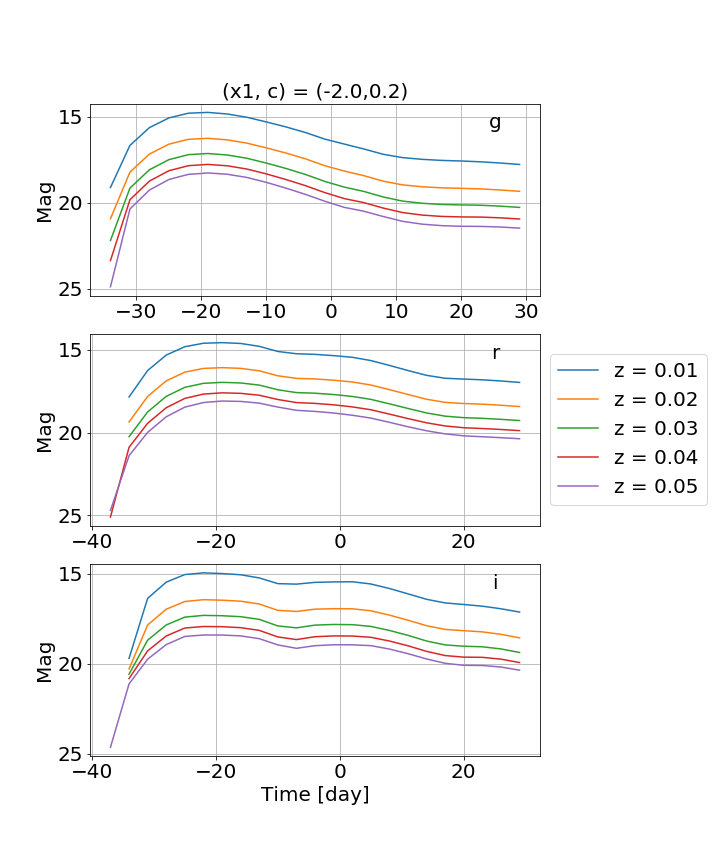
\includegraphics[width=0.9\textwidth]{LC_faint.png}
 \caption{Magnitude as a function of time and redshift for a faint type Ia supernovae and for $g$ (top), $r$ (middle) and $i$ (bottom) bands.}\label{fig:lcfaint}
\end{center}
\end{figure}

\begin{figure}[htbp]
\begin{center}
  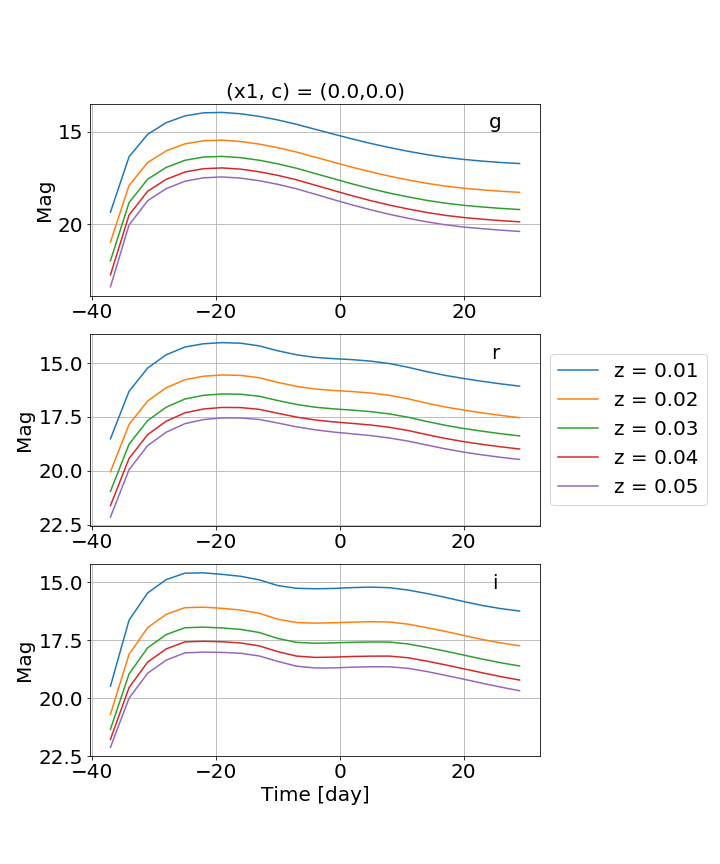
\includegraphics[width=0.9\textwidth]{LC_medium.png}
 \caption{Magnitude as a function of time and redshift for a medium type Ia supernovae and for $g$ (top), $r$ (middle) and $i$ (bottom) bands.}\label{fig:lcmedium}
\end{center}
\end{figure}

\begin{figure}[htbp]
\begin{center}
  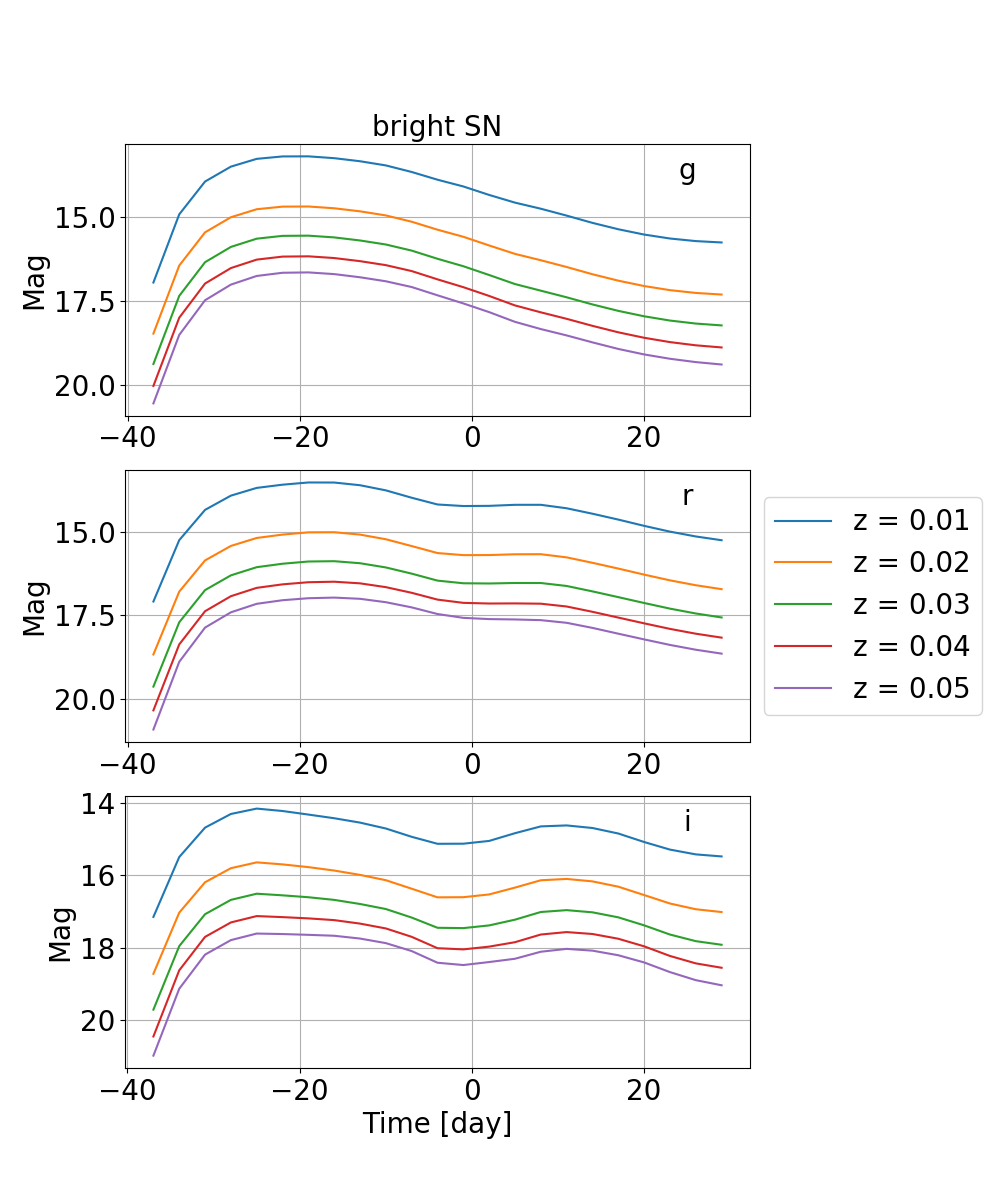
\includegraphics[width=0.9\textwidth]{LC_bright.png}
 \caption{Magnitude as a function of time and redshift for a bright type Ia supernovae and for $g$ (top), $r$ (middle) and $i$ (bottom) bands.}\label{fig:lcbright}
\end{center}
\end{figure}

\section{Illustration of the method}
\begin{figure}[htbp]
\begin{center}
  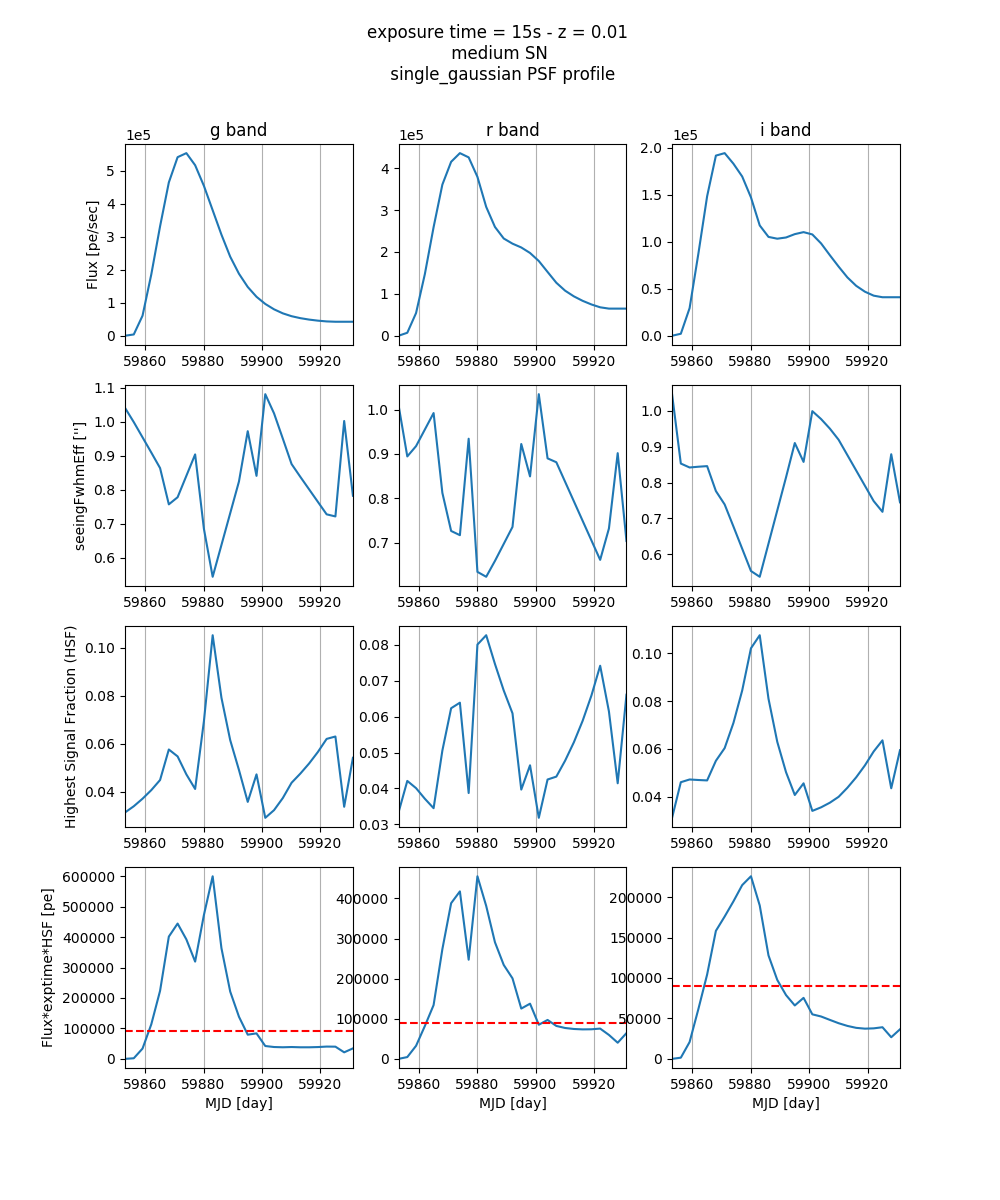
\includegraphics[width=0.8\textwidth]{procedure.png}
 \caption{Illustration of the method used to estimate saturation effects. To each LC simulated point (first row) corresponds a seeing (second row) from which a factor corresponding to the highest fraction of energy deposited in a pixel is estimated (third row). We multiply this factor by the exposure time (here 15s) and the flux to estimate (fourth row) the highest signal deposited (in pe) in a pixel.  LC points corresponding to saturation are removed if their fluxes are greater or equal the ccd full well ((red dotted line; 90 kpe).}\label{fig:method}
\end{center}
\end{figure}

\section{Saturation effects on flux distribution}

\begin{figure}[htbp]
\begin{center}
  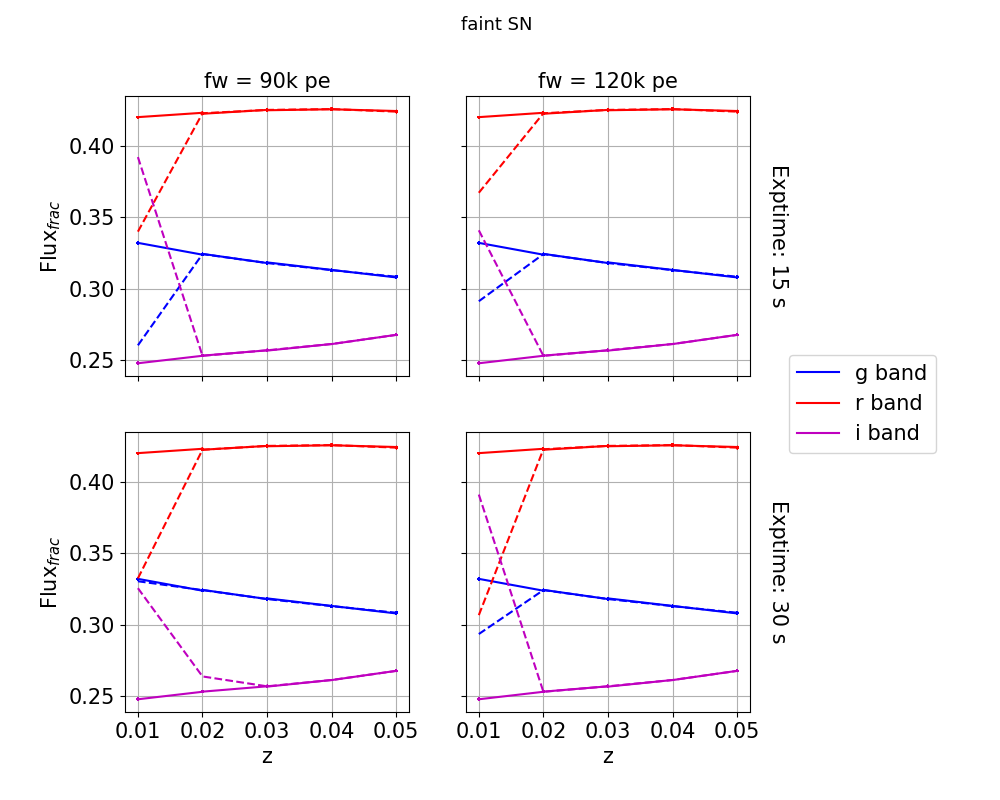
\includegraphics[width=0.9\textwidth]{Flux_faint.png}
 \caption{Saturation effect on flux distribution for a faint \sne. Flux fraction variations as a function of the redshift are given for $gri$ bands and four (exposure time, full well) configurations: (15s, 90k \pe) (top left),  (15s, 120k \pe) (top right), (30s, 90k \pe) (bottom left),  (30s, 120k \pe) (bottom right). All LC points have been considered to draw full lines. Dotted lines correspond to the case where saturated fluxes have been removed in the estimation (median values).}\label{fig:fluxfaint}
\end{center}
\end{figure}

\begin{figure}[htbp]
\begin{center}
  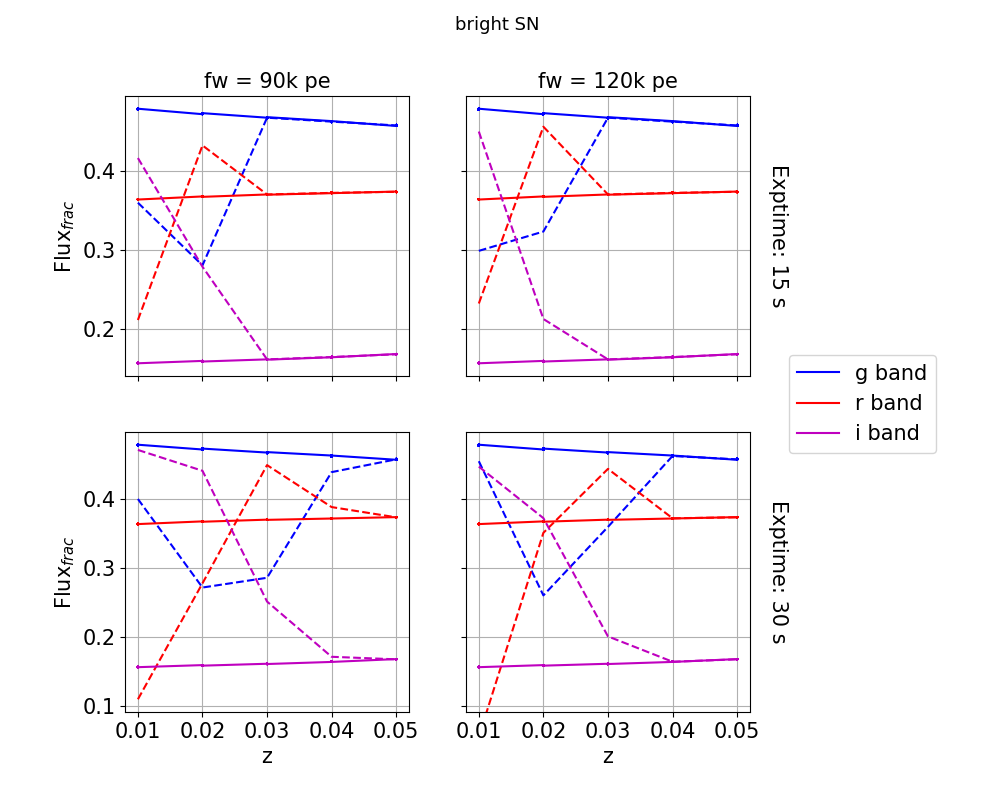
\includegraphics[width=0.9\textwidth]{Flux_bright.png}
  \caption{Saturation effect on flux distribution for a bright \sne. Flux fraction variations as a function of the redshift are given for $gri$ bands and four (exposure time, full well) configurations: (15s, 90k \pe) (top left),  (15s, 120k \pe) (top right), (30s, 90k \pe) (bottom left),  (30s, 120k \pe) (bottom right). All LC points have been considered to draw full lines. Dotted lines correspond to the case where saturated fluxes have been removed in the estimation (median values).}\label{fig:fluxbright}
  
\end{center}
\end{figure}
\newpage
\section{Saturation effects on Signal-to-Noise Ratio}

\begin{figure}[htbp]
\begin{center}
  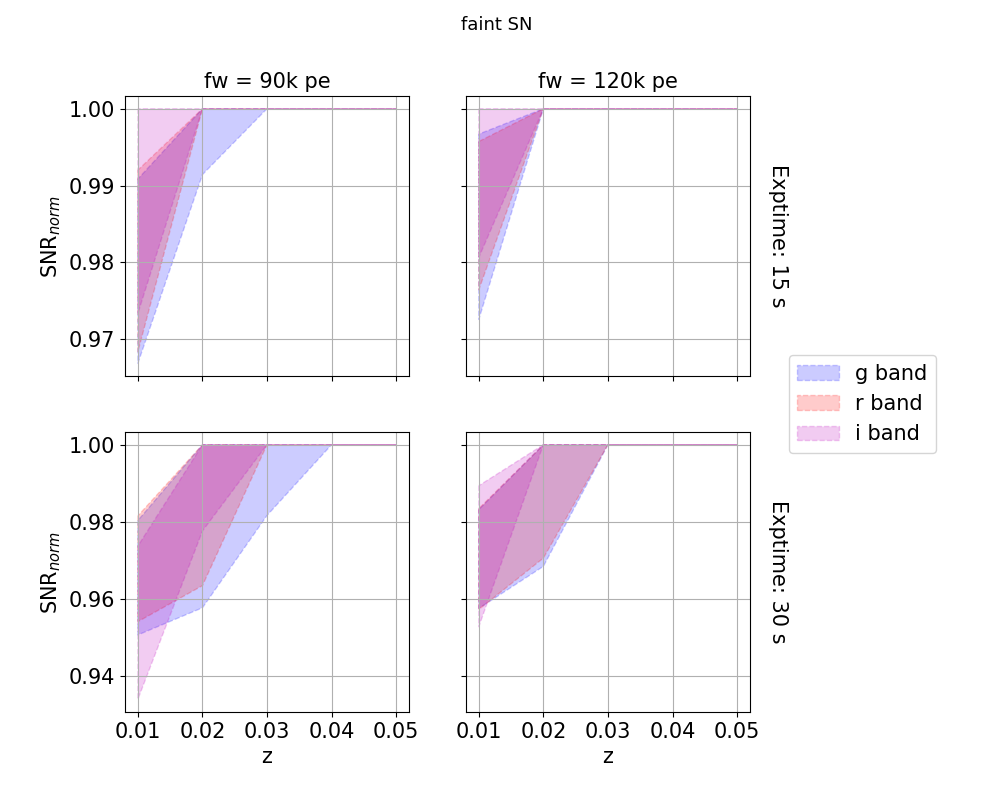
\includegraphics[width=0.9\textwidth]{SNR_faint.png}
 \caption{Saturation effect on Signal-to-Noise Ratio for a faint \sne. SNR (normalized to SNR values estimated without saturation included) variations as a function of the redshift are given for $gri$ bands and four (exposure time, full well) configurations: (15s, 90k \pe) (top left),  (15s, 120k \pe) (top right), (30s, 90k \pe) (bottom left),  (30s, 120k \pe) (bottom right),}\label{fig:snrfaint}
\end{center}
\end{figure}

\begin{figure}[htbp]
\begin{center}
  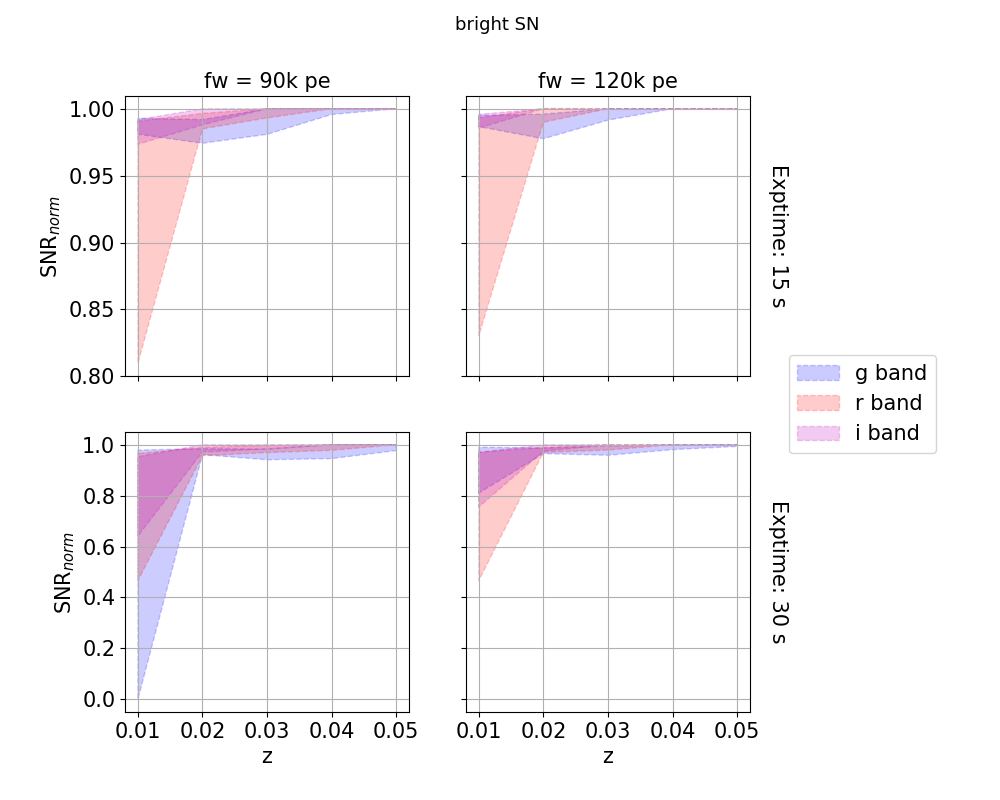
\includegraphics[width=0.9\textwidth]{SNR_bright.png}
 \caption{Saturation effect on Signal-to-Noise Ratio for a bright \sne. SNR (normalized to SNR values estimated without saturation included) variations as a function of the redshift are given for $gri$ bands and four (exposure time, full well) configurations: (15s, 90k \pe) (top left),  (15s, 120k \pe) (top right), (30s, 90k \pe) (bottom left),  (30s, 120k \pe) (bottom right),}\label{fig:snrbright}
\end{center}
\end{figure}
\newpage
\section{Saturation effects on \colorerr}

\begin{figure}[htbp]
\begin{center}
  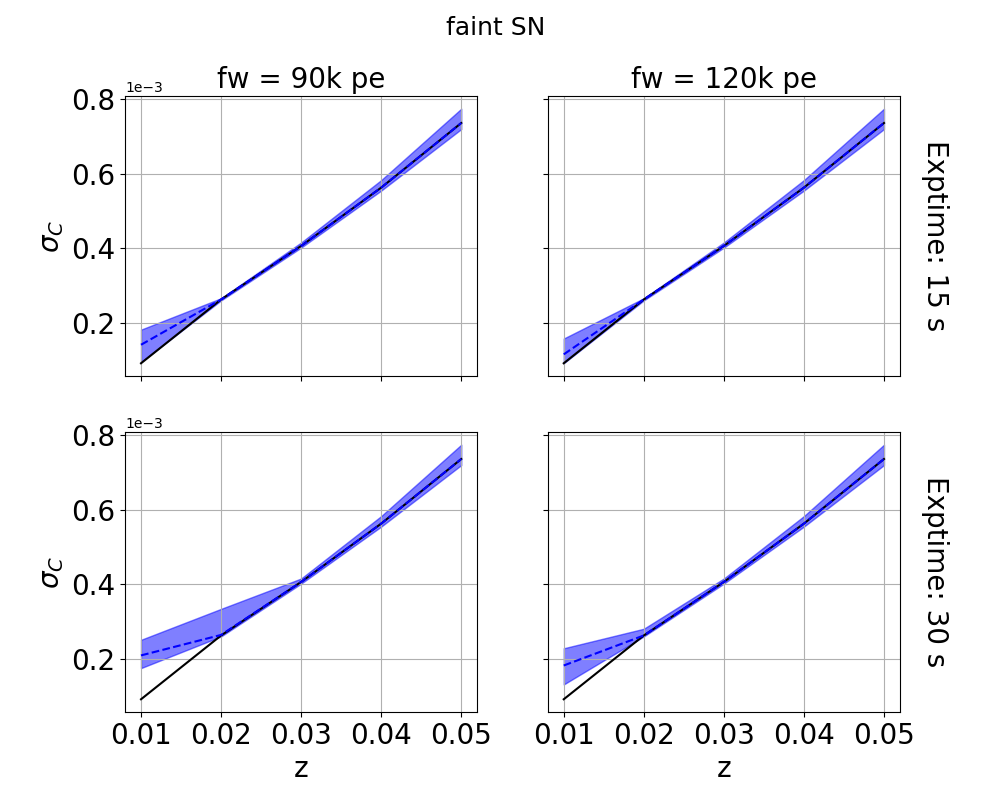
\includegraphics[width=0.9\textwidth]{sigmac_faint.png}
 \caption{Saturation effect on \colorerr~for a faint \sne. \colorerr~variations as a function of the redshift are given for $gri$ bands and four (exposure time, full well) configurations: (15s, 90k \pe) (top left),  (15s, 120k \pe) (top right), (30s, 90k \pe) (bottom left),  (30s, 120k \pe) (bottom right). Dotted lines correspond to median values if LC saturated points are removed from \colorerr~estimation. Full lines correspond to the case where all LC points are considered (median values).}\label{fig:sigmafaint}
\end{center}
\end{figure}

\begin{figure}[htbp]
\begin{center}
  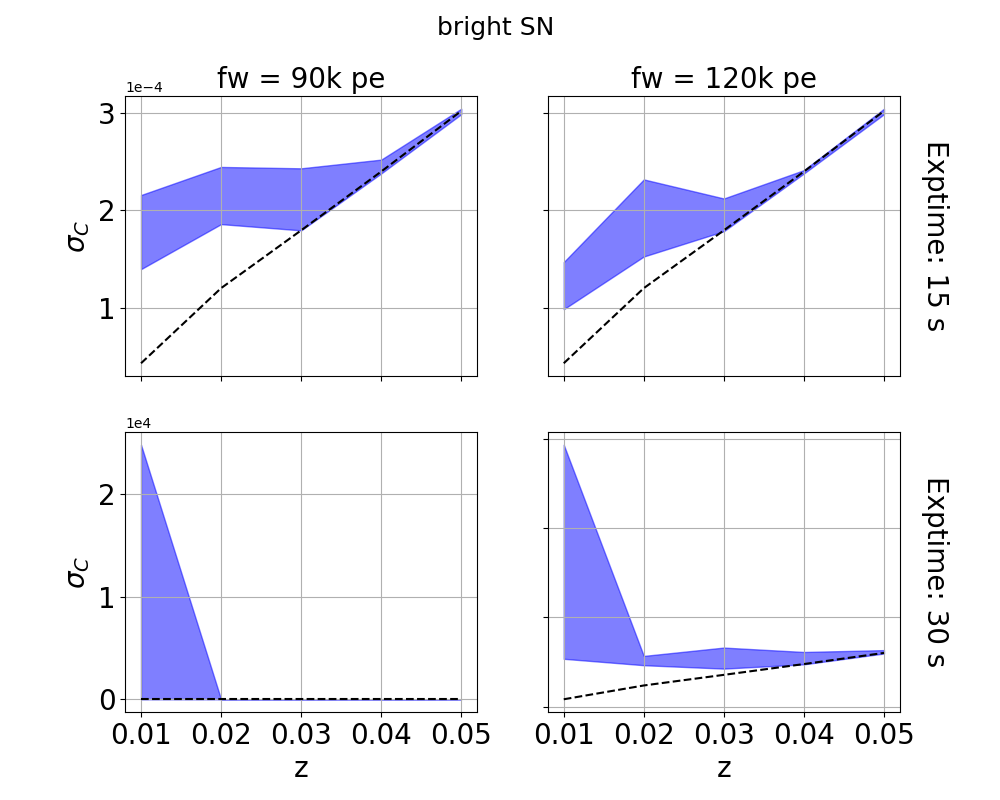
\includegraphics[width=0.9\textwidth]{sigmac_bright.png}
 \caption{Saturation effect on \colorerr~for a bright \sne. \colorerr~variations as a function of the redshift are given for $gri$ bands and four (exposure time, full well) configurations: (15s, 90k \pe) (top left),  (15s, 120k \pe) (top right), (30s, 90k \pe) (bottom left),  (30s, 120k \pe) (bottom right). Dotted lines correspond to median values if LC saturated points are removed from \colorerr~estimation. Full lines correspond to the case where all LC points are considered (median values).}\label{fig:sigmabright}
\end{center}
\end{figure}



\end{appendices}



